\subsection{Algorithmus}\label{subsec:splay-algorithmus}
Ein Splay-Tree ist ein Binärbaum, der beim Einfügen und Suchen von Elementen, diese jeweils an
die Wurzel befördert.
Dieser Vorgang wird Splaying gennant.

\paragraph{Splaying}
Ähnlich wie beim AVL-Baum wird wieder ein Knoten als Wurzel betrachtet.
Zunächst wird das gesuchte Element an diese Wurzel gebracht.
Dieser Prozess wird anschließend rekursiv auf die verbleibenden Knoten über der Wurzel angewendet,
bis das Element an der Wurzel des kompletten Baumes steht.

Es wird zwischen 3 Fällen unterschieden, die durch den Pfad von der Wurzel zu dem nach oben
zu befördernden Elementes definiert sind.
Alle Fälle haben jeweils ein symmetrisches Paar.
In Abbildung~\ref{fig:splayinCase} ist jeweils eines der Paare dargestellt.
In Klammern ist der symmetrische Fall angegeben.
Die Wurzel \verb|x| ist dabei jeweils die, die nach oben befördert werden soll.
%\begin{enumerate}
%    \item Zig-Zag: L/L oder R/R
%    \item Zig-Zig: L/R oder R/L
%    \item Zig: L oder R
%\end{enumerate}

\begin{figure}[hbt]
    \centering
    \subfloat[\centering Zig Zig: L/L (R/R)]{
    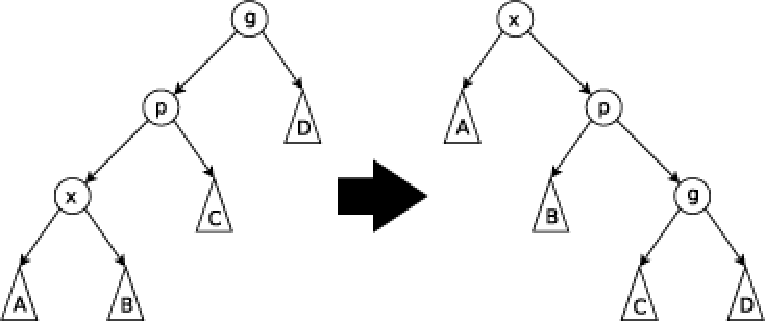
\includegraphics[width = 0.45\textwidth]{img/splay/zigzig}}
    \qquad
    \subfloat[\centering Zig Zag: L/R (R/L)]{
    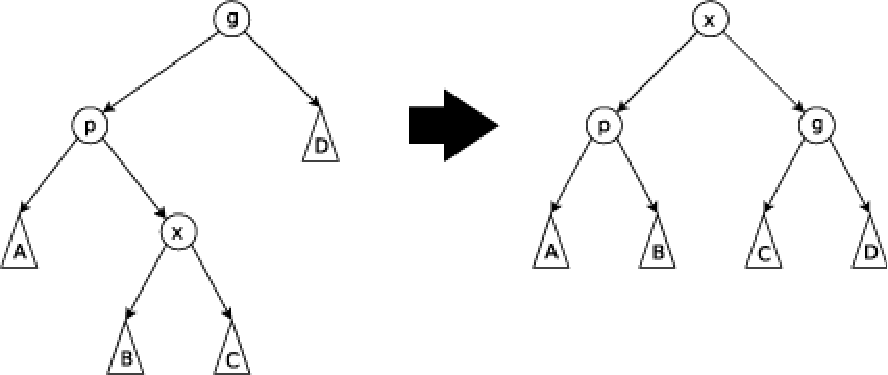
\includegraphics[width = 0.48\textwidth]{img/splay/zigzag}}
    \qquad
    \subfloat[\centering Zig: L (R)]{
    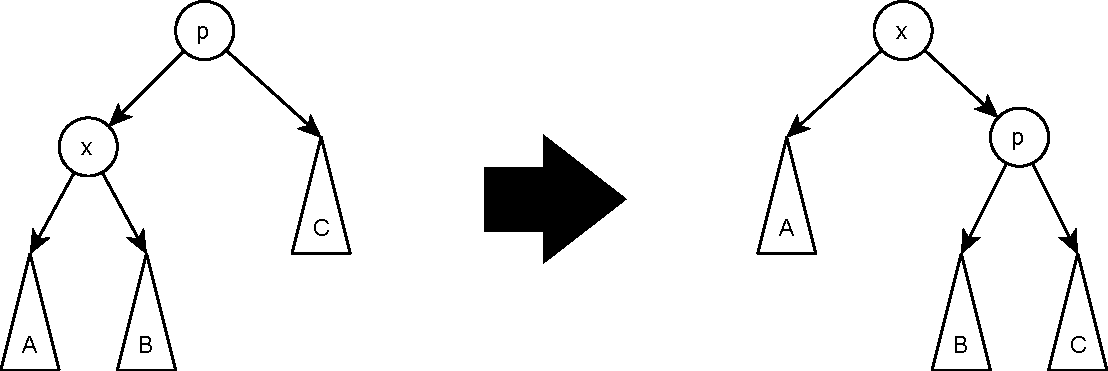
\includegraphics[width = 0.52\textwidth]{img/splay/zig}}
    \caption{Splaying Vorgang}\label{fig:splayinCase}
\end{figure}

\subsection{Entwurf}\label{subsec:splay-entwurf}

\paragraph{InitBT, IsEmptyBT, EqualBT, PrintBT}
Wie beim AVL-Baum kann auch hier die Implementation des Binärbaumes verwendet werden.
Lediglich InitBT wird wieder um das Zurücksetzen der Counter erweitert.
PrintBT ist identisch zu der in Abschnitt~\ref{subsec:entwurf2} beschrieben Methode.

\paragraph{IsBT}
Bei dem AVL-Baum wurde \nameref{par:avl-isBT} um das Überprüfen der AVL-Bedingung erweitert.
So konnte die korrekte Arbeitsweise des AVL-Baumes sichergestellt werden.
Bei dem Splay-Tree lässt sich die Korrektheit vom Splaying jedoch nicht überprüfen, da die
Datenstruktur selber keine Informationen über die Zugriffe auf Elemente speichert.
In \verb|IsBT(BTree)| werden also lediglich die Voraussetzungen des Binärbaumes überprüft,
somit kann die Implementation vom Binärbaum übernommen werden.

\paragraph{FindBT}\label{par:splay-findBT}
Beim Finden eines Elementes wird dieses an die Wurzel des Baumes befördert.
Dafür wird zunächst top-down das gesuchte Element gefunden, wobei der Pfad
bottom-up hoch gegeben wird.
Als Erstes wird \verb|HERE|, danach \verb|L| oder \verb|R| zurückgegeben.
Beim zweiten Schritt ist das gesuchte Element zwei Elemente entfernt, kann also über zwei
Kanten erreicht werden.
Nun wird die entsprechende Doppelrotation durchgeführt.
Das gesuchte Element steht jetzt an dem Knoten, der gerade als Wurzel betrachtet wird, somit wird
als Pfad \verb|HERE| zurückgegeben.
Dies wird rekursiv fortgeführt, bis die Wurzel des Baumes erreicht wird.
Der Vorgang ist in Abbildung~\ref{fig:splayFind} dargestellt.
\begin{figure}[hbt]
    \centering
    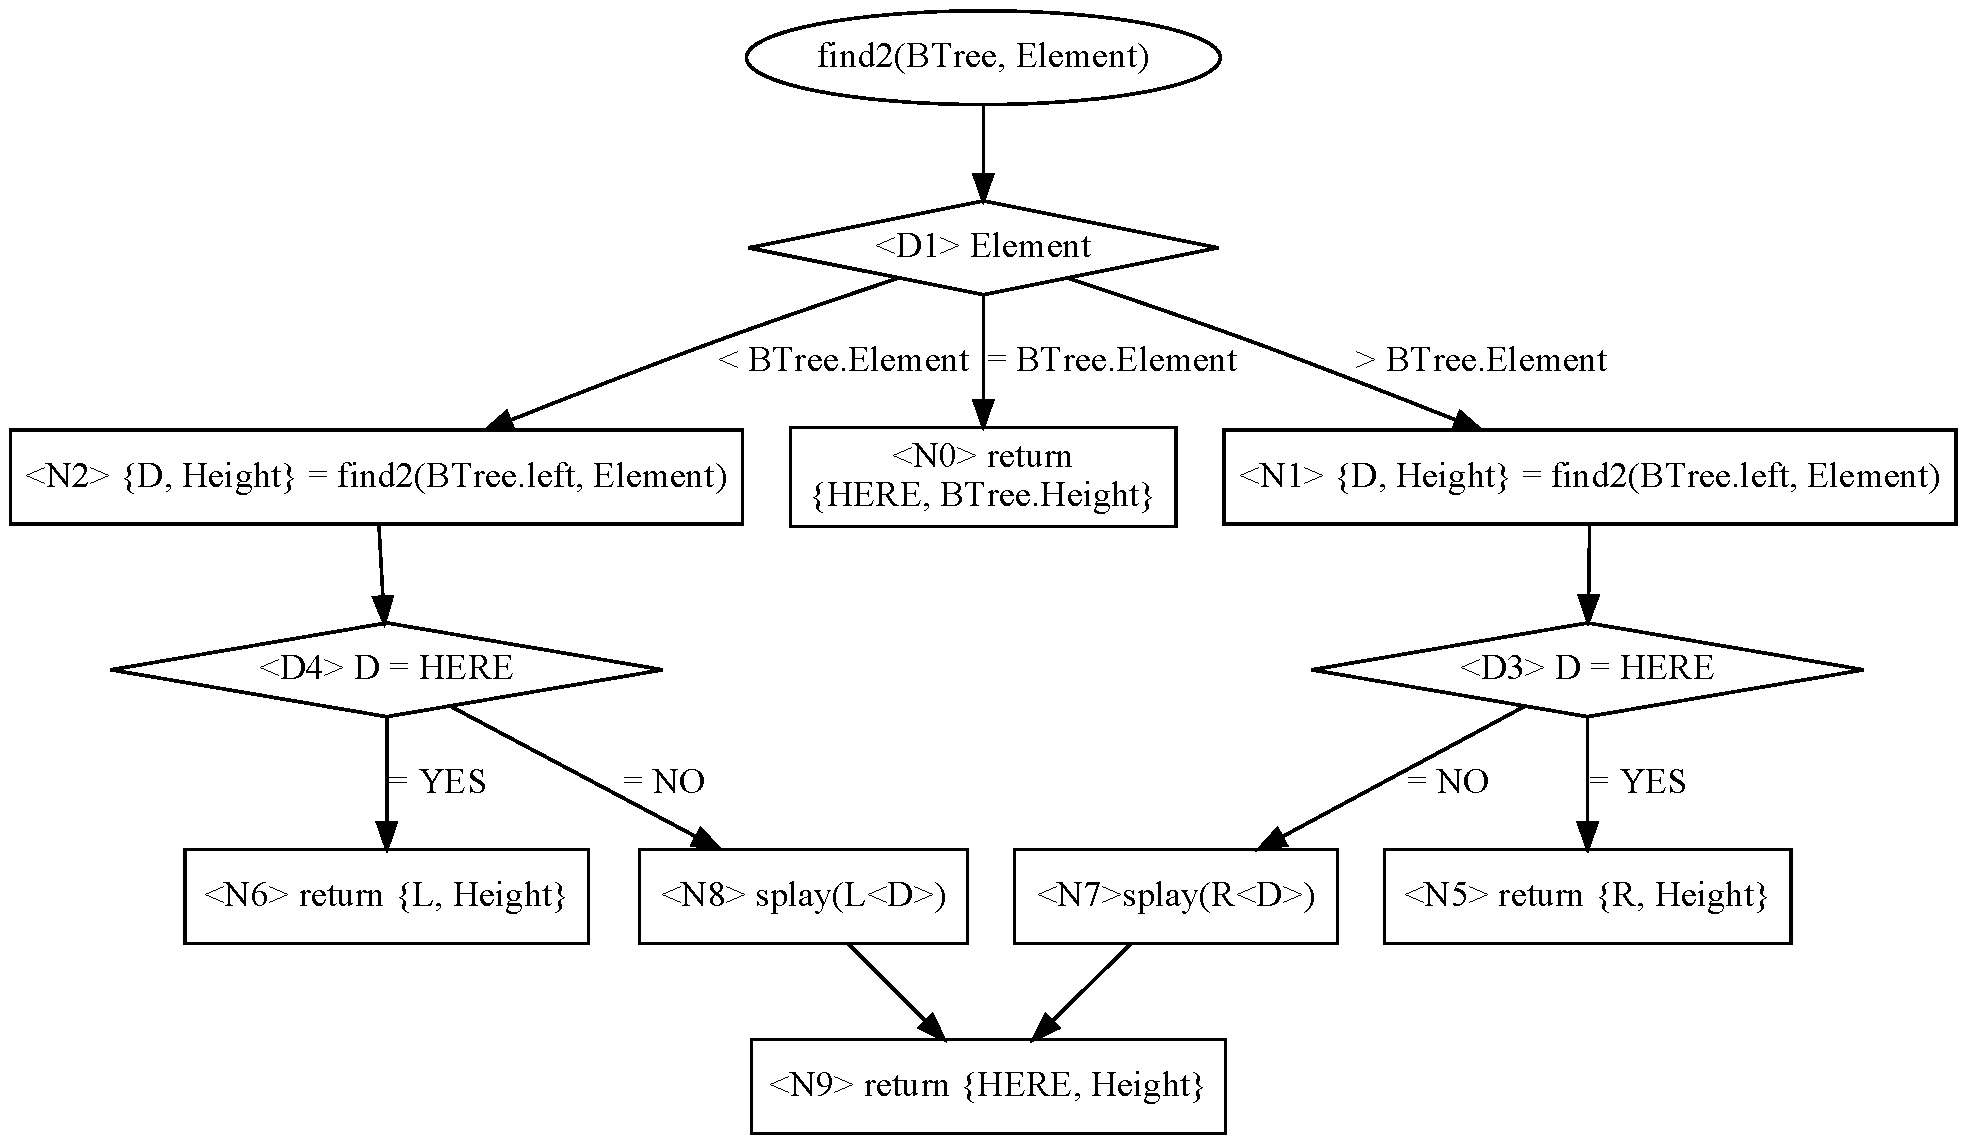
\includegraphics[width=\textwidth]{img/splay/splayFind2}
    \caption{FindBT}
    \label{fig:splayFind}
\end{figure}

In der Abbildung ist der Fall, dass das gesuchte Element nicht im Baum vorhanden ist, präteriert.
Hierfür kann der Pfad z.B. als \verb|NOTFOUND| zurückgegeben werden.
Falls bei der Überprüfung dessen \verb|NOTFOUND| vorliegt, werden keine Rotationen ausgeführt.

Da immer zwei Nachfolger betrachtet werden, ist es möglich, dass am Ende das gesuchte Element
am linken oder rechtem Kind vom Wurzelknoten steht.
Um dies zu überprüfen, wird die eben beschriebene Methode in eine Wrapper-Methode umhüllt.
Dort kann getestet werden, ob am Ende \verb|HERE| zurückgegeben wurde.
Falls dies der Fall ist, wird ein Zig (Einfachrotation) ausgeführt.
Anschließend steht das gesuchte Element an der Wurzel.
Dies ist in Abbildung~\ref{fig:splayFind2} dargestellt.
\begin{figure}[hbt]
    \centering
    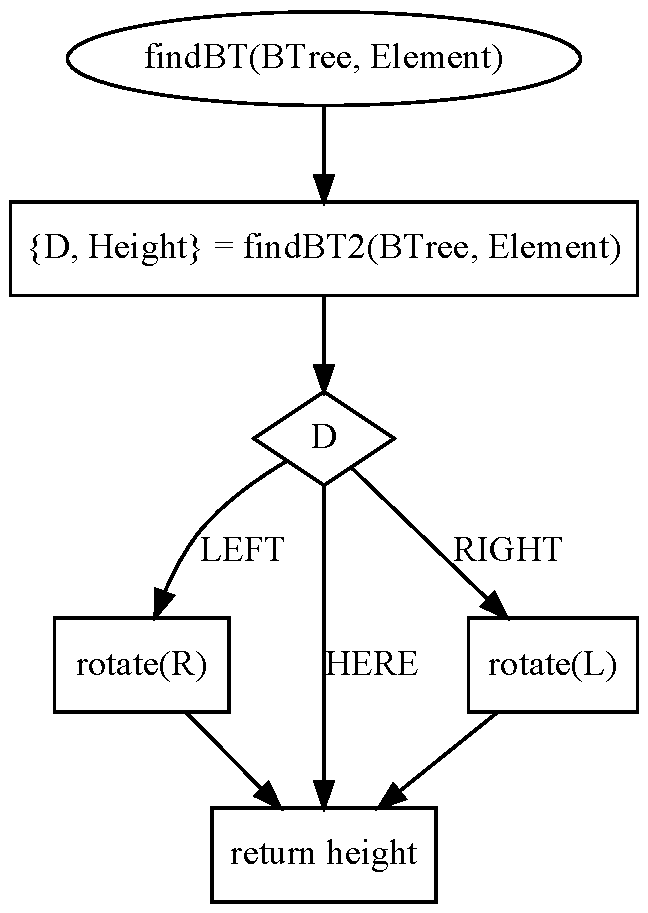
\includegraphics[width=0.35\textwidth]{img/splay/splayFind}
    \caption{FindBT Wrapper}
    \label{fig:splayFind2}
\end{figure}

\paragraph{FindTP}
Alternativ kann beim Finden eines Elementes dieses nur um einen Knoten nach oben bewegt werden.
Zunächst wird das Element gefunden, anschließend eine Zig-Operation durchgeführt.
Um dies zu realisieren, wird, sobald das Element gefunden wurde, ein Flag zurückgegeben, welches
signalisiert, dass rotiert werden soll.
Dieses Flag wird nur einmal zurückgegeben, sodass insgesamt nur einmal rotiert wird.

\paragraph{InsertBT}
Beim Einfügen eines Elementes wird dieses an die Wurzel befördert.
Dies kann dadurch realisiert werden, dass das Element zunächst wie bei einem Binärbaum
eingefügt, anschließend mithilfe von \nameref{par:splay-findBT} an die Wurzel befördert wird.
Diese Implementation hat den Nachteil, dass der Baum insgesamt zweimal durchlaufen wird.
Zur Optimierung ist es möglich, beide Schritte in einem Durchlauf durchzuführen: Zunächst top-down
das Element einfügen, dann, mithilfe von Rotationen, bottom-up das Element zur Wurzel bringen.
Dabei ist letzteres wie bei \nameref{par:splay-findBT} zu realisieren,
die Höhe muss dabei nicht zurückgegeben werden.

\paragraph{DeleteBT}
